\section{实验配置与结果}
\label{sec:experiment}
\subsection{配置及数据划分}
\begin{table}[htbp]\centering
\caption{确定性合成实验配置}\label{tab:config}
\begin{tabular}{ll}\toprule
项目 & 设置\\\midrule
样本总数 & 120\\
目标异常数 / 正常数 & 12 / 108\\
异常比例 & 10\%\\
周期基线 & 式\eqref{eq:baseline}\\
随机种子 & 不使用随机数\\
训练集 / 验证集 & 不适用，无学习过程\\
评估集 & 全部 120 个合成观测\\
固定阈值 / 残差阈值 & 22 / 1.8、1.55\\
统计精度 & 双精度计算，表格保留四位小数\\\bottomrule
\end{tabular}\end{table}
所有规则在生成数据之前即已固定，没有基于结果搜索最优阈值。为便于复现，生成脚本一次性写出原始数据、指标表、混淆矩阵、完整数据附录和两幅 PNG 图片。表格与图片消费同一份内存数据，避免手工复制数值造成不一致。

\subsection{时间序列可视化}
\begin{figure}[htbp]\centering
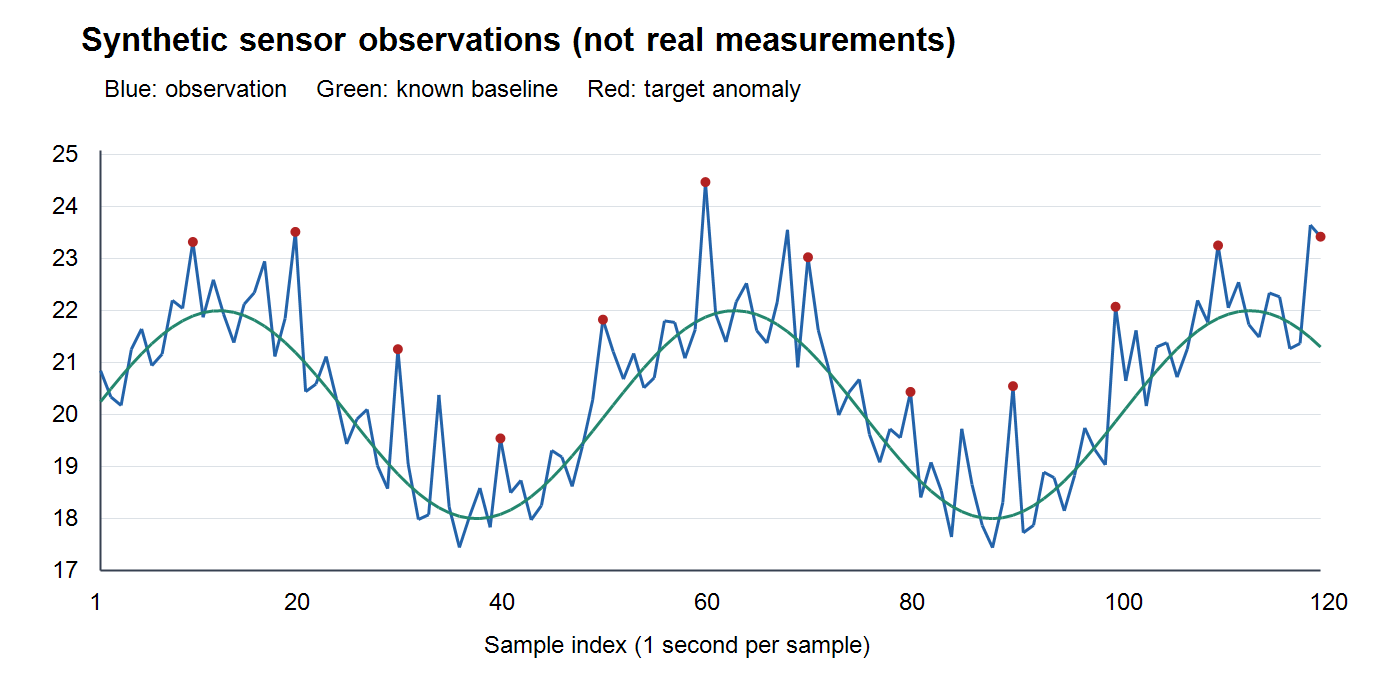
\includegraphics[width=0.96\linewidth]{figures/signal.png}
\caption{合成观测与已知基线。红点表示目标异常；横轴为样本下标，纵轴为合成温度。图片内英文标签用于避免绘图阶段依赖中文字体。}\label{fig:signal}
\end{figure}
图\ref{fig:signal}中的周期项使固定阈值在高基线区域更容易触发，在低基线区域则可能漏过目标异常。残差规则消除了已知周期项，但仍可能将非目标扰动判为异常。注意，“消除周期项”只是在公式已知的前提下相减，不涉及模型训练或实际信号分解。

\subsection{定量比较}
\begin{table}[htbp]\centering
\caption{合成数据上的检测指标}\label{tab:metrics}
\begin{tabular}{lrrrr}\toprule
规则 & Accuracy & Precision & Recall & $F_1$\\\midrule
A & 0.8250 & 0.3043 & 0.5833 & 0.4000\\
B & 0.9333 & 0.7000 & 0.5833 & 0.6364\\
C & 0.9333 & 0.6667 & 0.6667 & 0.6667\\
\bottomrule\end{tabular}\end{table}
\begin{table}[htbp]\centering
\caption{可独立复算的混淆矩阵计数}\label{tab:confusion}
\begin{tabular}{lrrrr}\toprule
规则 & TP & TN & FP & FN\\\midrule
A & 7 & 92 & 16 & 5\\
B & 7 & 105 & 3 & 5\\
C & 8 & 104 & 4 & 4\\
\bottomrule\end{tabular}\end{table}
表\ref{tab:metrics}使用式\eqref{eq:f1}等定义计算；表\ref{tab:confusion}给出全部整数计数，便于独立复算。每一行都必须满足 $\mathrm{TP}+\mathrm{FN}=12$、$\mathrm{TN}+\mathrm{FP}=108$，且四项计数之和为 120。

\begin{figure}[htbp]\centering
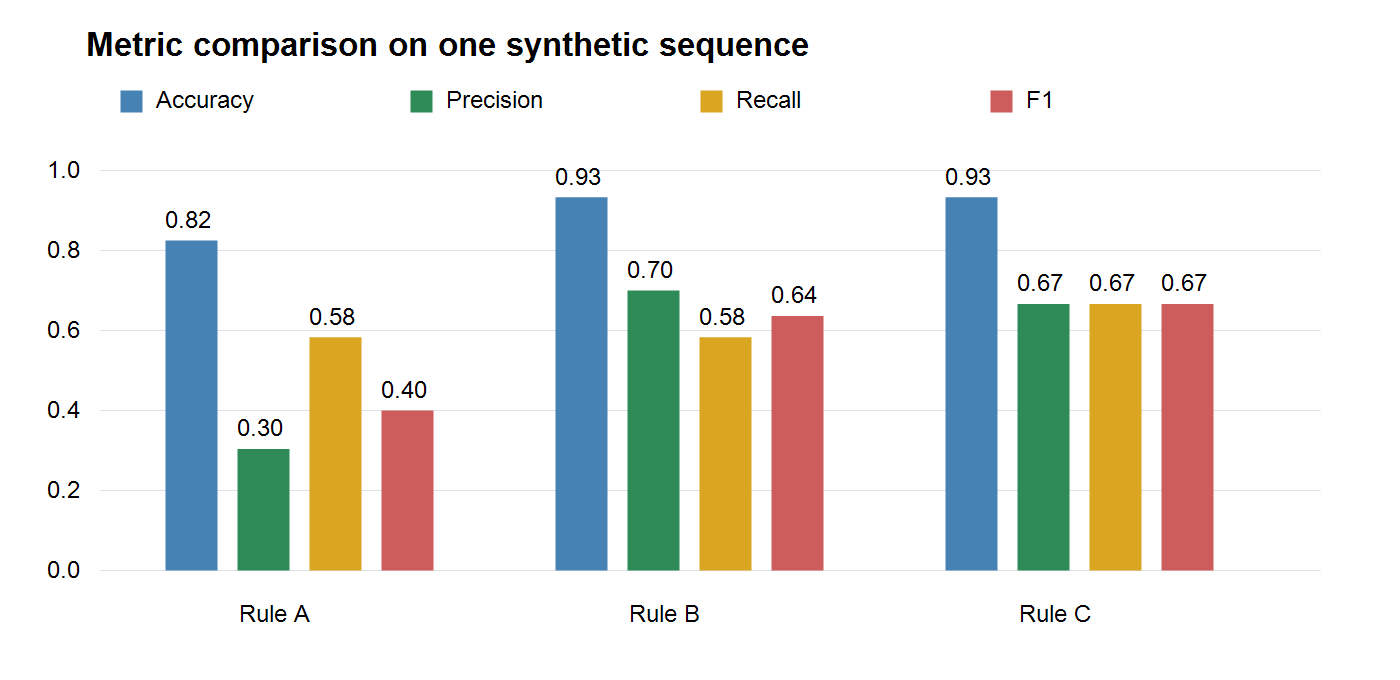
\includegraphics[width=0.86\linewidth]{figures/metrics.png}
\caption{三种检测规则的指标比较。数值范围为 0 至 1，与表\ref{tab:metrics}使用同一计算结果。}\label{fig:metrics}
\end{figure}
对 B 与 C 而言，降低阈值使预测正例集合只增不减，因此召回率不应下降，误报数也不应下降；精确率和 F1 则不保证单调。图\ref{fig:metrics}用于检查这种数值关系及图片嵌入是否正确，不用于替代逐点计数。

\subsection{可复算样本与错误分析}
\begin{table}[htbp]\centering\small
\caption{前十二个观测点}\label{tab:sample}
\begin{tabular}{rrrrrrrr}\toprule
$i$ & $b_i$ & $x_i$ & $r_i$ & $y_i$ & A & B & C\\\midrule
1 & 20.249 & 20.844 & 0.595 & 0 & 0 & 0 & 0\\
2 & 20.495 & 20.341 & 0.153 & 0 & 0 & 0 & 0\\
3 & 20.733 & 20.177 & 0.555 & 0 & 0 & 0 & 0\\
4 & 20.959 & 21.255 & 0.296 & 0 & 0 & 0 & 0\\
5 & 21.170 & 21.649 & 0.479 & 0 & 0 & 0 & 0\\
6 & 21.363 & 20.943 & 0.420 & 0 & 0 & 0 & 0\\
7 & 21.535 & 21.164 & 0.371 & 0 & 0 & 0 & 0\\
8 & 21.683 & 22.198 & 0.515 & 0 & 1 & 0 & 0\\
9 & 21.805 & 22.043 & 0.238 & 0 & 1 & 0 & 0\\
10 & 21.898 & 23.321 & 1.423 & 1 & 1 & 0 & 0\\
11 & 21.962 & 21.872 & 0.089 & 0 & 0 & 0 & 0\\
12 & 21.995 & 22.595 & 0.600 & 0 & 1 & 0 & 0\\
\bottomrule\end{tabular}\end{table}
表\ref{tab:sample}列出前十二个点，涵盖正常点和第一个目标异常。更详细的失败分析可在 CSV 中筛选 $y_i\ne\hat y_i$。对 A 应同时观察基线所处相位，对 B、C 应观察扰动叠加后的残差，不应把每次误报都解释为程序错误。

\subsection{编译与复现协议}
主文件为 \texttt{main.tex}，章节通过 \texttt{input} 组织，图片使用相对路径。首次排版后执行 BibTeX，再运行两轮 pdfLaTeX；目录、引用及参考文献稳定后才作为最终产物。编译全过程不需要网络、Shell Escape 或外部图片服务\cite{lolReproduce2026}。
